\documentclass[a4paper,10pt]{article}
\ifdefined\forprint
    \usepackage[width=21.6cm,height=30.3cm,center]{crop}
\fi
\usepackage[utf8]{inputenc}

\usepackage[margin=2cm,headheight=26pt,includeheadfoot]{geometry}

\usepackage[ngerman]{babel}
\usepackage[german=quotes]{csquotes}

\usepackage{nameref}
\usepackage{microtype}
\usepackage{float}
\usepackage{siunitx}
\sisetup{
    locale = DE,
    binary-units,
    detect-all,
    per-mode = symbol %enables m/s instead of ms^-1
}
\AtBeginDocument{\DeclareSIUnit{\kWh}{kWh}}

\usepackage{caption} %for \caption*
\usepackage{hhline}
\usepackage{tabularx}
\usepackage{array}
\usepackage{calc}
\usepackage{multicol}
\usepackage{multirow}
\usepackage{parskip}
\usepackage{booktabs}

\usepackage{fancyhdr}
\pagestyle{fancy}
\setlength{\headheight}{48pt}
\renewcommand{\headrulewidth}{0pt}

\usepackage{xcolor,colortbl}
\usepackage{makecell}

\usepackage[symbol*]{footmisc}
\renewcommand{\thefootnote}{\fnsymbol{footnote}}
\renewcommand{\thempfootnote}{\fnsymbol{mpfootnote}}

\usepackage{color}
\usepackage{enumitem}

\usepackage{pdfpages}

% Word-Stealth-Modus, kann aber kein Omega
%\usepackage[scaled]{helvet}

\usepackage[inline,nomargin]{fixme}

\definecolor{fxnote}{rgb}{0.8000,0.0000,0.0000}
\colorlet{fxnotebg}{yellow}

\definecolor{boxgray}{rgb}{0.33,0.33,0.33}
\definecolor{boxred}{rgb}{0.8,0,0}
\usepackage{tcolorbox}
\title{}
\author{}

\renewcommand{\familydefault}{\sfdefault}

\newcommand{\hint}[1]{\begin{tcolorbox}[colback=boxgray,colframe=black,coltext=
white,title=Hinweis]#1\end{tcolorbox}}

\newcommand{\warn}[1]{\begin{tcolorbox}[colback=boxred,colframe=red,coltext=
white,title=Warnung]#1\end{tcolorbox}}

\newcommand{\gfx}[1]{\includegraphics[width=\linewidth]{#1}}

\newcommand*{\fullref}[1]{\hyperref[{#1}]{\ref*{#1}~\nameref*{#1}}}

\fancyhf{}
\fancyhead{\colorbox{boxgray}{
    \makebox[\dimexpr\linewidth-2\fboxsep][l]{
        
\includegraphics[height=1cm]{./img/logo}\hfill\color{white}\Huge\raisebox{.5ex}{\thepage}
        }
    }
}

\usepackage{hyperref}
\usepackage{qrcode}

\appto\UrlNoBreaks{\do\.\do\:\do\/\do\_}

\usepackage{hyphenat}

\begin{document}
\pagestyle{empty}
\begin{titlepage}
	\vspace*{-3.08cm}
	\colorbox{boxgray}{\makebox[\dimexpr\linewidth-2\fboxsep][c]{
\includegraphics[width=0.6\textwidth]{./img4/logo}}}
	\vfill
	\begin{center}
		\Huge
		Betriebsanleitung\\\vspace{0.25cm}WARP4 Ladesäule\\\vspace{1cm}
		\large
		Version 1.0.0\\\vspace{0.25cm}
		\today
	\end{center}
	\vfill
	\begin{center}
		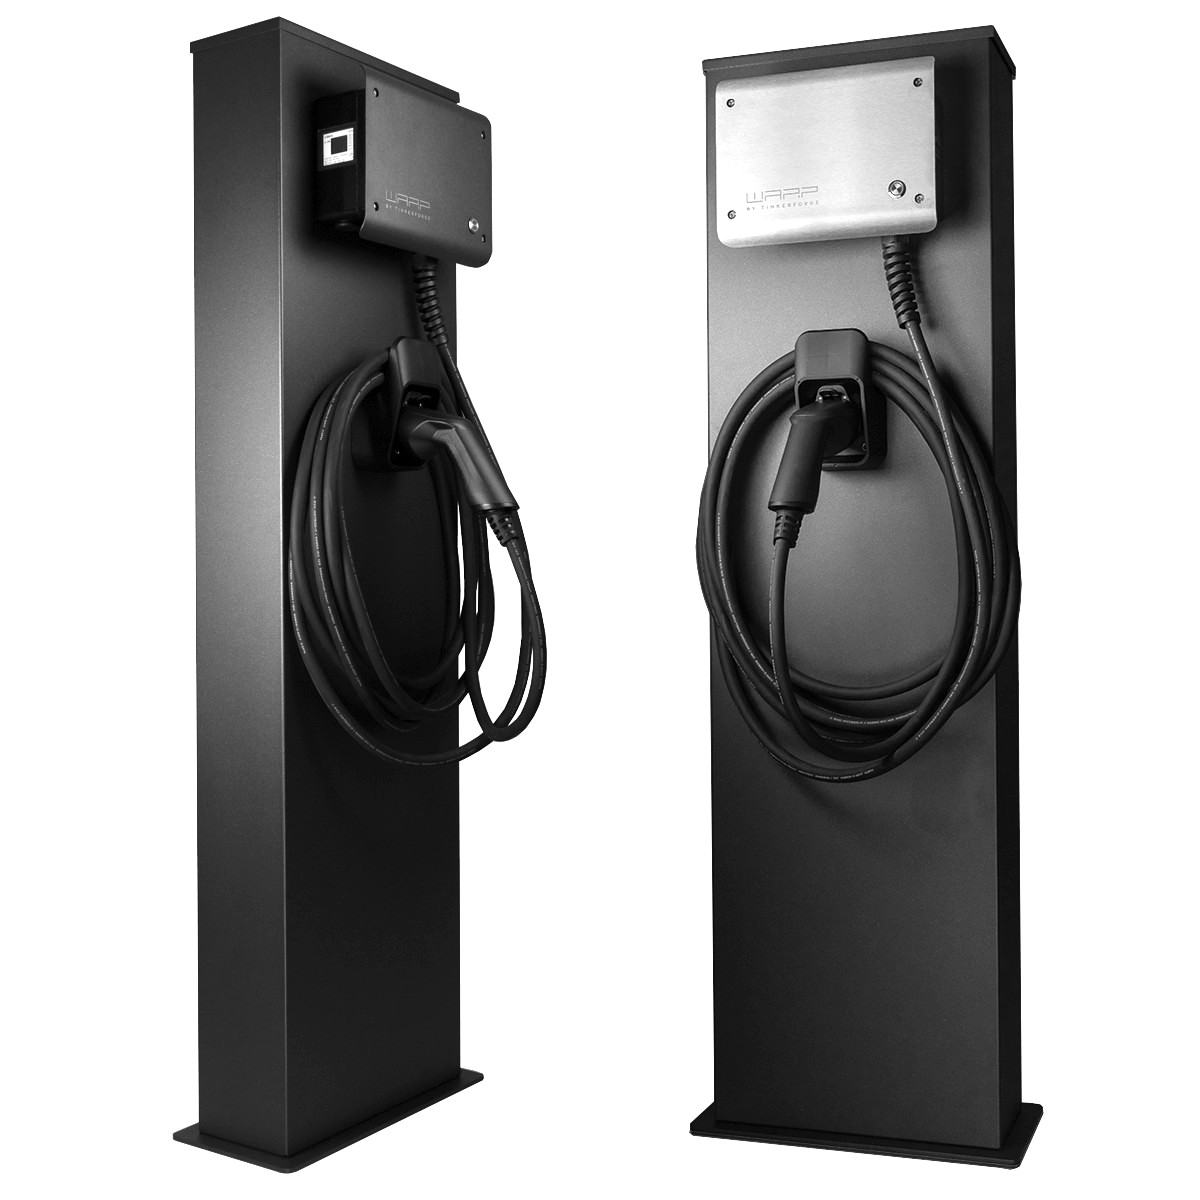
\includegraphics[width=0.6\linewidth]{./img4/Stand_Versions.jpg}
	\end{center}
\end{titlepage}
\newpage
\newpage
\pagestyle{fancy}
\begin{multicols*}{2}
	\tableofcontents \section{Einführung}
	\subsection{Vorwort} Vielen Dank, dass du
	dich für eine WARP4 Ladesäule von Tinkerforge entschieden hast!

	\enquote{WARP} steht
	für \textbf{W}all \textbf{A}ttached
	\textbf{R}echarge \textbf{P}oint. Mit der WARP4 Ladesäule
	erhältst du eine hochqualitative und langlebige Ladesäule, mit der du dein
	Elektrofahrzeug laden kannst. Die nachfolgende Betriebsanleitung gibt dir
	alle notwendigen Informationen zu Sicherheit, Montage, Installation, Betrieb
	und Wartung der Ladesäule.

	\subsection{Beschreibung}

	Die WARP4 Ladesäule ist in mehreren Varianten verfügbar:
	Ausgelegt für die Montage von einem oder zwei WARP4 Charger Wallboxen sowie
	mit Verteilergehäuse oder ohne.
	\par
	Die Ladesäule besteht aus \SI{2.0}{\milli\meter}
	verzinktem Stahl der zusätzlich in DB703 pulverbeschichtet wurde. Mit der Schutzklasse IP54
	ist die Säule für den
	Außenbereich geeignet. Die mitgelieferte Montagehilfe, die die Befestigungsschrauben im
	richtigen Abstand positioniert, ermöglicht es das Betonfundament
	vorzubereiten und die Ladesäule später einfach aufzusetzen.
	\par
	Nach der Fertigstellung des Fundaments und gegebenenfalls weiteren
	notwendigen Erdarbeiten wird die Ladesäule montiert.
	Über die geteilte Rückwand kann die Zuleitungen einfach erreicht und 
	die Ladesäule bequem angeschlossen werden.
	\par
	Ein optional bestellbarer
	Verteilerkasten ist mit Hutschiene und Klemmen ausgestattet und wird mit
	vorgefertigen Anschlussleitungen geliefert. Der große Verteilerkasten
	bietet die Möglichkeit zusätzliche Hardware wie LTE-Router, Ethernet Switche
	o.ä. in der Ladesäule geschützt zu montieren.

\vspace{-0.2cm}
	\section{Sicherheitshinweise}
\vspace{-0.2cm}
	\subsection{Allgemein}
	Die WARP4 Ladesäule ist so konstruiert, dass ein sicherer Betrieb gewährleistet ist,
	wenn sie korrekt installiert wurde, in einem einwandfreien technischen Zustand
	ist und diese Betriebsanleitung befolgt wird. \hint{Die Ladesäule darf nur von einer ausgewiesenen Elektrofachkraft installiert
		werden.}
\vspace{-0.2cm}
	\subsection{Bestimmungsgemäße Verwendung}
	Die Ladesäule dient zur Aufnahme von WARP4 Charger Wallboxen auf einer freien
	Fläche, bei der eine Wandmontage nicht möglich oder nicht gewünscht ist. 
	Es dürfen ausschließlich WARP4 Charger
	an der Ladesäule montiert werden. Den Installations- und
	Verwendungshinweisen der verwendeten WARP4 Charger ist Folge zu leisten.
	Diese sind in der Betriebsanleitung der WARP4 Charger zu finden.

	Die Ladesäule ist in zwei Produktvarianten erhältlich:
	\begin{itemize}
		\item Aufnahme für eine WARP4 Charger Wallbox.
		\item Aufnahme für zwei WARP4 Charger Wallboxen.
	\end{itemize}
	Die Variante für zwei Wallboxen verfügt über Aussparungen und
	Befestigungspunkte für die zweite Wallbox auf der Rückseite. 
	Es ist nicht zulässig, nur die frontseitige Wallbox zu montieren und die
	zweite Wallbox dann nicht zu montieren.
\vspace{-0.2cm}
	\subsection{Allgemeine Sicherheitshinweise}

	Die WARP4 Ladesäule wurde gemäß den relevanten Sicherheits- und Umweltvorschriften und -bestimmungen
	entwickelt, hergestellt, geprüft und dokumentiert. Sie darf nur in technisch einwandfreiem Zustand verwendet werden.

	Störungen, die die Sicherheit von Personen oder des Geräts beeinträchtigen,
	sind sofort von einer autorisierten Elektrofachkraft nach den national geltenden Regeln beheben zu lassen.

	\warn{Nichtbeachtung der Sicherheitshinweise kann zu Lebensgefahr,
	Verletzungen und Schäden am Gerät führen! Der Hersteller lehnt jede Haftung
	für daraus resultierende Ansprüche ab!
	\\
	\\
	\textbf{Elektrische Gefahr!}\\
	Die Montage, erste Inbetriebnahme und Wartung der Ladestation darf nur von
	einer ausgebildeten, qualifizierten und befugten Elektrofachkraft
	durchgeführt werden, die dabei für die Beachtung der bestehenden Normen und
	Installationsvorschriften verantwortlich ist. Halte die angeführten Vorgaben 
	für die Standortauswahl und die baulichen Voraussetzungen ein! Abweichungen 
	zu den Standortvorgaben können zu Tod, schweren Körperverletzungen oder 
	Sachschäden führen, wenn die entsprechenden Vorsichtsmaßnahmen nicht 
	getroffen werden!
	} 


	\subsection{Öffnen der Ladesäule}

	\begin{center}
		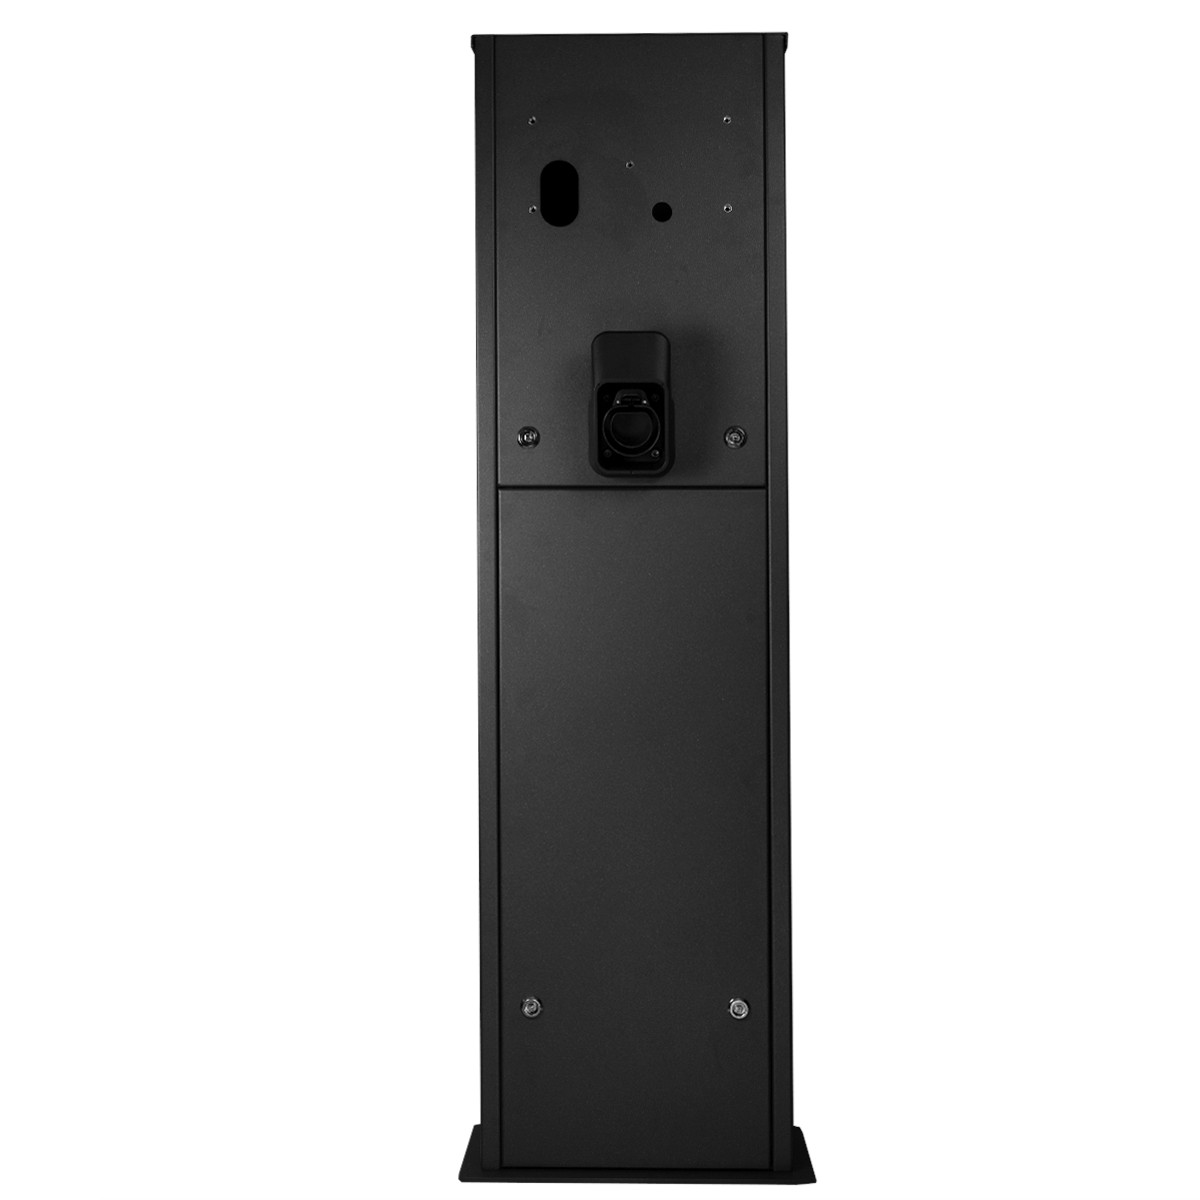
\includegraphics[width=\linewidth]{./img4/stand-back.jpg}
	\end{center}

	Die Ladesäule besitzt eine geteile Rückseite. Diese sind mit
	Verschlussriegeln ausgestattet, die mittels der mitgelieferten
	Schaltschrankschlüssels geöffnet werden können. Zum Öffnen und Entfernen des
	oberen Teils muss immer zuerst der untere Teil entfernt werden.

	\section{Montage und Installation}
	\subsection{Montage}
	\subsubsection{Lieferumfang}
	Im Lieferumfang der Ladesäule befinden sich (abhängig ob Säule für eine
	Wallbox oder zwei Wallboxen):
	\begin{itemize}
		\item Ladesäule mit Fuß
		\item Rückseite (Oberer Teil) inkl. 2x Verschlussriegel
		\item Rückseite (Unterer Teil) inkl. 2x Verschlussriegel
		\item Vormontierte Montagehilfe bestehend aus:
			\begin{itemize}
				\item 2x Montagehilfe-Blech
				\item 4x M8 Gewindestangen
				\item 4x Unterlegscheiben
				\item 16x M8 Muttern
			\end{itemize}
		\item Schaltschrankschlüssel
		\item 1x/2x Kabelhalterungen inkl. 4x M6x16mm Innensechskantsschrauben
		\item 4x/8x Innensechskantschrauben M6x35mm zur Befestigung der Wallboxen
		\item 2x/3x Erdungsschraubenset, je
		\begin{itemize}
			\item 1x M6x16mm Innensechskant
			\item 2x M6 Unterlegscheibe
			\item 1x M6 Fächerscheibe
		\end{itemize}
		\item Diese Betriebsanleitung
	\end{itemize}

	Optional kann die Ladesäule mit einem Verteilergehäuse und Kabelanschlusset
	geliefert werden. In diesem Fall sind folgende Komponenten zusätzlich
	enthalten:
	\begin{itemize}
		\item Verteilergehäuse vorbestückt für eine oder zwei Wallboxen
				\begin{itemize}
				\item Verteilergehäuse
				\item Hutschiene
				\item 1x/2x Klemmenblock
				\item RJ45 Hutschienen-Patchkabelverbinder
				\item 4x M6x10mm Innensechskantschrauben zur Befestigung
				\item 1x/2x RJ45 Patchkabel 1.5m
			\end{itemize}
			\item 1x/2x Wallboxanschlussleitung
			\item 1x Erdungsanschlussleitung Verteilerbox
			\item 1x/2x Erdungsanschlussleitung Wallbox
	\end{itemize}
\vspace{-0.1cm}
	\subsubsection{Montageort}
	Folgende Anforderungen müssen zur Montage der WARP4 Ladesäule erfüllt sein:
	\begin{itemize}
		\item Der Einbauort muss alle Anforderungen erfüllen, die in der
		WARP4 Charger Bedienungsanleitung aufgeführt sind.
		\item Bei Installation der Ladesäule an einer Straße oder einem
		öffentlichen Parkplatz, offen oder überdacht, muss ein entsprechender
		Anfahr-/Rammschutz angebaut werden.
		\item Sollen mehrere Ladesäulen nebeneinander installiert werden, muss
		der Abstand zwischen den einzelnen Ladesäulen mindestens \SI{200}{\milli\meter} betragen.
		\item Die Oberfläche muss vollständig plan sein.
	\end{itemize}

    \hint{Die Ladesäule nicht auf Asphalt installieren! Auf Asphalt ist die
	Standsicherheit nicht gewährleistet.}


	\subsubsection{Herstellung des Fundaments}
    Zur sicheren Installation der Ladesäule wird ein Betonfundament empfohlen.
	Auslegung, Konstruktion und Ausführung des Fundaments sind Aufgabe des
	Herstellers des Betonfundaments und gegebenenfalls den örtlichen Gegebenheiten
	anzupassen.

	Auf Seite~\pageref{appendix_base} findet sich eine
	Abbildung zur Herstellung des Fundaments. Die Größe des Betonfundaments ist als
	Mindestgröße anzusehen um einen sicheren Stand zu gewährleisten.

	Die Montagehilfe wird fertig aufgebaut mitgeliefert und kann direkt im Betonfundament positioniert werden.
	Bei der Montage sind die angegebenen Maße einzuhalten. 

	Es darf sich kein Wasser am Fundament ansammeln, dieses muss abfließen können. Die
	Stromversorgungskabel, ein Erdungskabel und gegebenenfalls vorhandene Netzwerkkabel müssen in der Mitte
	des Betonfundaments austreten und eine überstehende Länge von mindestens
	\SI{1500}{\milli\meter} haben. Dazu ist in der Montagehilfe eine
	Ovale-Aussparung mit Außenabmessungen von 110 × \SI{55}{\milli\meter}.
	Der Fundamenthersteller muss
	für einen ausreichenden Schutz der Kabel sorgen. Schutzhüllen müssen mindestens
	\SI{300}{\milli\meter} aus dem Beton herausreichen. Ein Erdungsanschluss ist
	zwingend erforderlich.

	\subsubsection{Montage der Ladesäule}
	Nachdem das Betonfundament gegossen wurde und ausgehärtet ist, kann
	die Ladesäule montiert werden. Zuvor sollten die Rückseiten
	entfernt werden. Die bei der Montagehilfe
	eingesetzten oberen M8 Muttern (4 Stück) und die Unterlegscheiben müssen nun wieder losgeschraubt werden,
	damit die Gewinde offen liegen. Anschließend kann die Stele mittig über den
	Kabeln, die aus dem Fundament ragen, positioniert werden. Die
	einbetonierte Montagehilfe sorgt für die korrekte Position der
	Befestigungsschrauben. Nach dem Auftstellen der Stele auf die Schrauben kann diese
	mittels der zuvor entfernten Unterlegscheiben und Muttern auf das Fundament
	geschraubt werden.

	Auf Seite~\pageref{appendix_base} findet sich eine
	Abbildung zu diesem Arbeitsschritt.

	\subsubsection{Montage des Kabelhalters}

	\begin{center}
		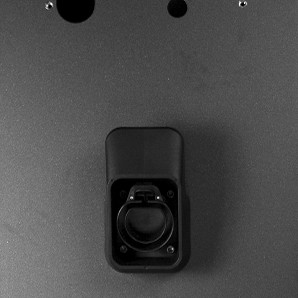
\includegraphics[width=0.5\linewidth]{./img4/cable-hook.jpg}
	\end{center}

	Je nach Variante der Ladesäule werden 1-2 Kabelhalter mitgeliefert. Diese
	werden mit den mitgelieferten M6x16mm Innensechskantschrauben unterhalb der Wallbox
	befestigt. Die Verschraubung erfolgt von außen durch den Kabelhalter.

	\subsection{Elektrische Installation}
	Der elektrische Anschluss der Wallboxen erfolgt für jede Wallbox separat.
	Die Hinweise der Elektroinstallation der WARP4 Charger aus deren
	Betriebsanleitung sind zu beachten.

	\subsubsection{Anforderungen an die Elektroinstallation}
	Die Anforderungen an die Elektroinstallation der gewählten WARP4
	Charger Wallboxen sind zu beachten. Diese sind der mitgelieferten
	Betriebsanleitung der Wallbox zu entnehmen.

	\subsubsection{Erdung}
	Als Erdungssternpunkt für die Ladesäule dient eine M6x16mm Schraube in der
	Fußplatte der Ladesäule. An dieser Schraube laufen alle Erdungsleitungen
	zusammen.
	
	\begin{center}
		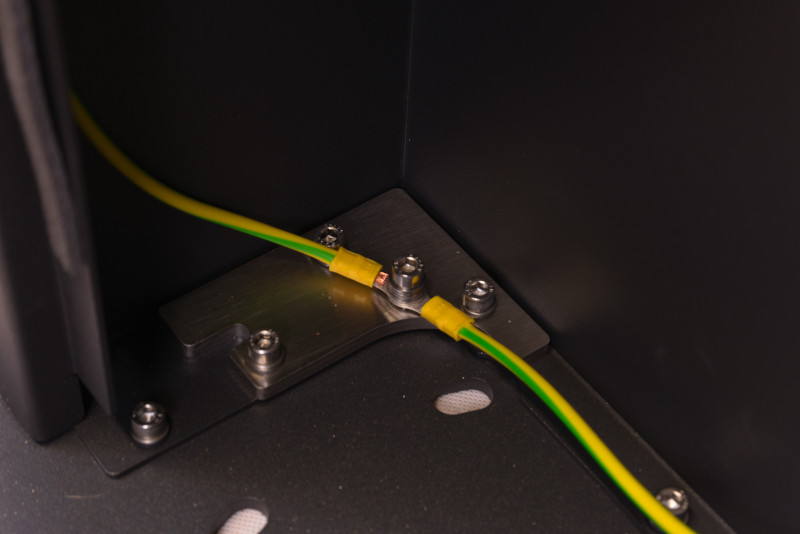
\includegraphics[width=\linewidth]{./img4/earth_star.jpg}
	\end{center}

	Diese M6 Schraube muss extern mit Erde verbunden werden. Wird die Verteilerbox
	eingesetzt, so liegt hierfür ein Erdungskabel M6 Ringschuh auf Aderendhülse
	bei. Die Erdungsverbindung erfolgt hierbei über die Erdungsklemme in der
	Verteilerbox und damit über die Versorgungszuleitung. 
	Wird keine Verteilerbox eingesetzt, so muss die Erde hier
	direkt angeschlossen werden.

	\begin{center}
		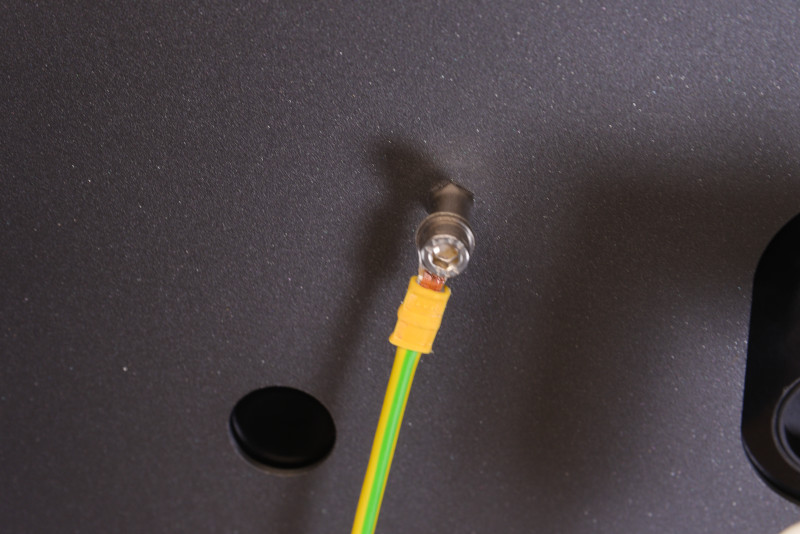
\includegraphics[width=\linewidth]{./img4/earth_wb.jpg}
	\end{center}

	Von dieser Erdungsschraube wird eine Erdungsleitung zur M6 Mutter gezogen,
	die sich in der Säule mittig hinter der Wallbox befindet. Die Erdungsleitung wird innen
	in der Säule mittels einer M6x16mm Schraube und Fächer- sowie
	Unterlegscheiben befestigt. Für Ladesäulen mit zwei Wallboxen, wird je eine
	Erdungsleitung zur Wallbox auf der Vorderseite als auch zur Wallbox auf der
	Rückseite (oberes Rückenteil) gezogen. An beiden Teilen ist dann je eine M6
	Mutter vorhanden.

	\subsubsection{Wallbox}
	Zur Montage an der Säule muss die Wallbox von einer Kabeleinführung von der
	Unterseite auf eine Kabeleinführung auf der Rückseite umgebaut werden. Wird
	die Säule mit der optional angebotenen Verteilerbox bestellt, so werden
	entsprechend konfektionierte Anschlussleitungen mitgeliefert. Es bietet sich an diese
	zuerst in der Wallbox zu installieren und mit der Kabelverschraubung zu
	fixieren. Selbiges gilt für Steuer- und Netzwerkleitungen.
	\par
	Anschließend kann die Wallbox mit den installierten Leitungen vor die Säule
	gehangen werden. Zu Befestigung werden die vier mitgelieferten M6x35mm
	Innensechskantschrauben verwendet.

	\subsubsection{Verteilergehäuse}

	\begin{center}
		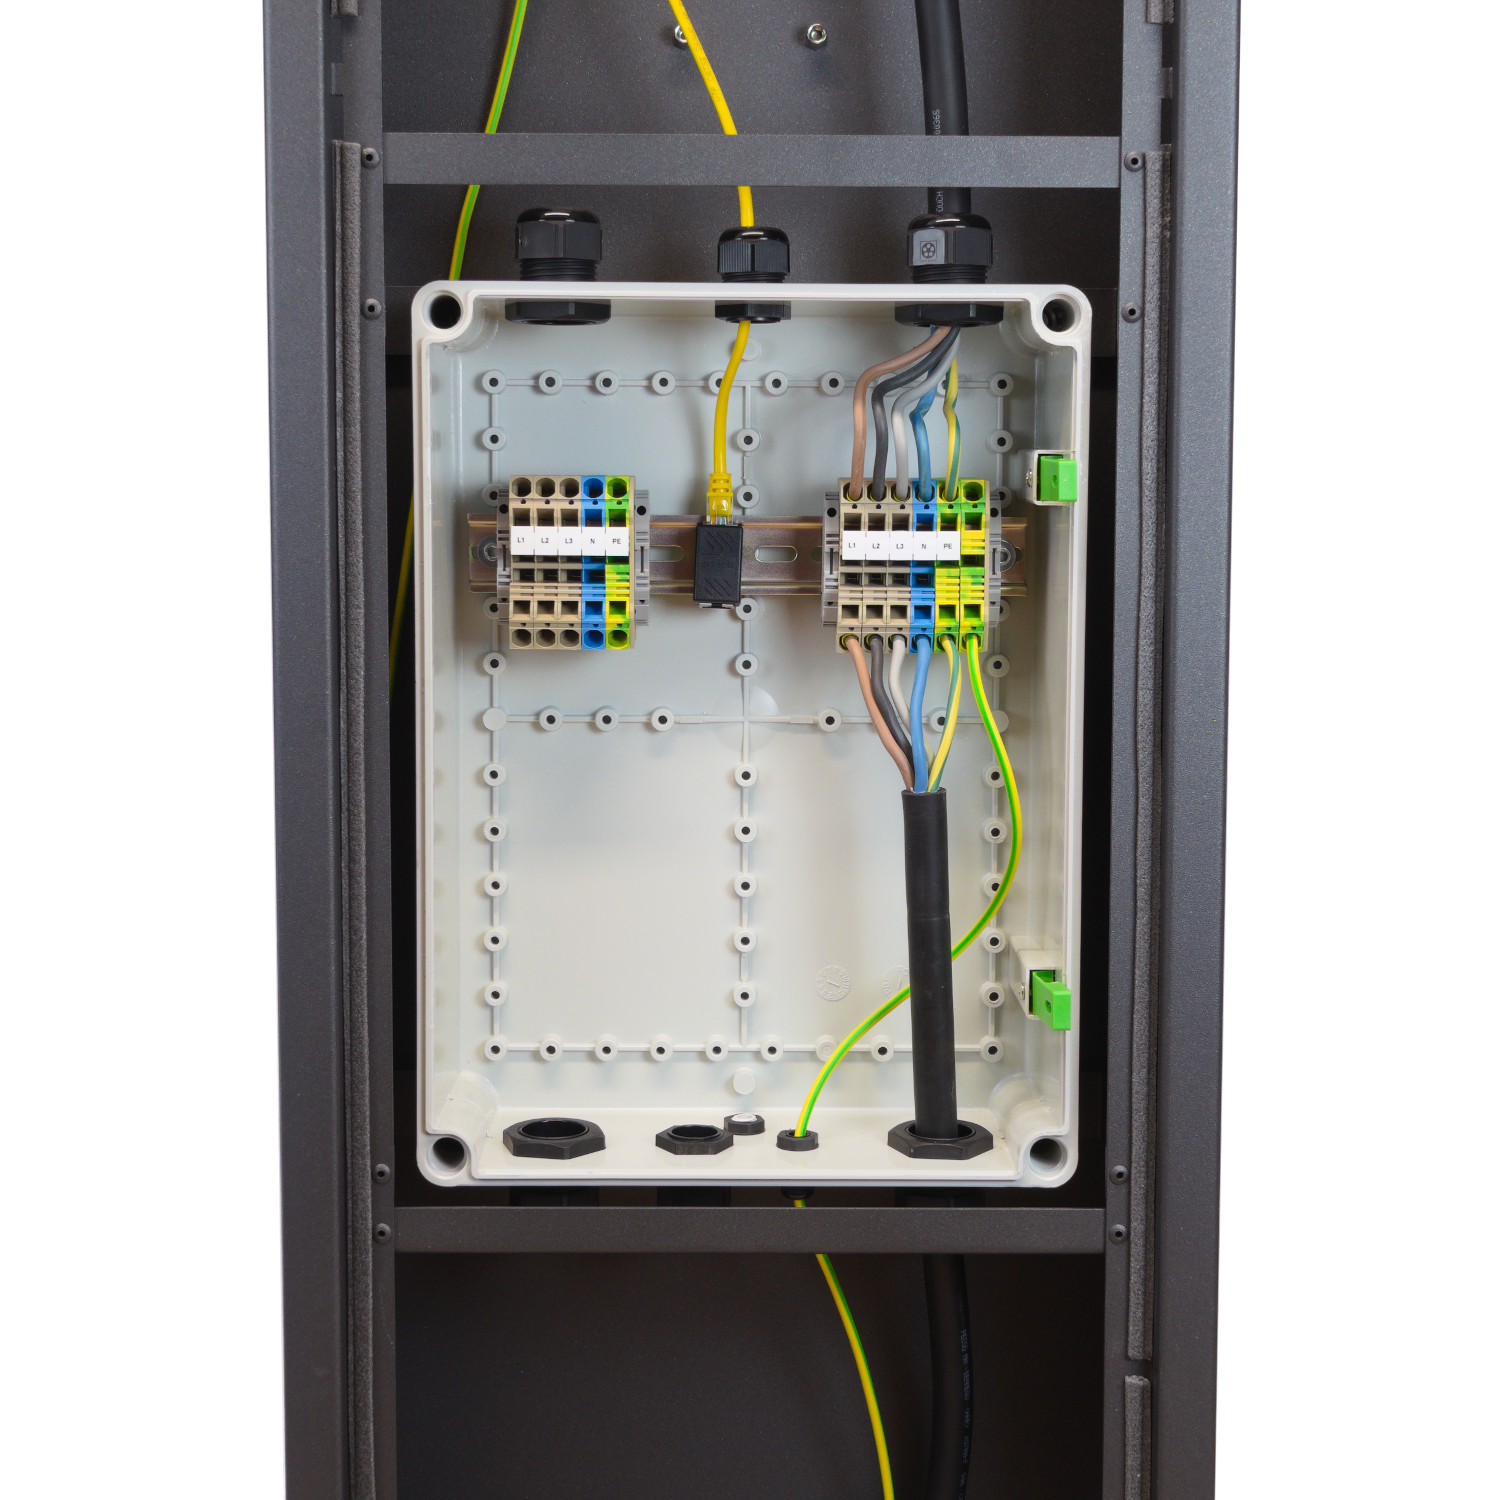
\includegraphics[width=\linewidth]{./img4/box.jpg}
	\end{center}

	Im Verteilergehäuse befinden sich Klemmen vom Typ SRK 10
	oder vergleichbar. Es können ein- und mehrdrähtige Leiter mit einem Querschnitt von bis zu
	\SI{16}{\square\milli\meter} und Leiter mit Aderendhülse mit einem
	Querschnitt von bis zu \SI{10}{\square\milli\meter} angeschlossen werden.
	Die Abisolierlänge beträgt \SI{10}{\milli\meter}. Der Anschluss erfolgt
	anhand der Beschriftung der Klemmen im Verteilergehäuse.

	Anschließend sind die in der Betriebsanleitung des WARP4 Chargers geforderten Prüfungen für die
	Wallboxen durchzuführen.

	\subsubsection{RJ45 - Ethernet}
	Das Verteilergehäuse dient ebenfalls zum Anschluss der Ethernetleitungen.
	Im Gehäuse können die bestehenden Ethernetleitungen der Wallbox
	angeschlossen werden. Dazu werden passende Patchkabel und einen
	Patchkabelverbinder für die Hutschiene mitgeliefert.

	\section{Inbetriebnahme}
	Eine Inbetriebnahme der eigentlichen Ladesäule erfolgt nicht, sondern eine 
	Inbetriebnahme der verbauten WARP4 Charger. Dazu finden sich weitere Informationen in der
	Betriebsanleitung der Wallboxen.

	\section{Wartung und Reinigung}
	\subsection{Wartung}
	Eine Wartung der Ladesäule ist nicht notwendig.

	\subsection{Reinigung}
	\warn{\textbf{Gefahr! Hochspannung}\\Gefahr von tödlichen elektrischen
	Stromschlägen. Die Ladesäule und die Wallboxen niemals mit einem Hochdruckreiniger oder einem ähnlichen Gerät reinigen.}
	\begin{itemize}
		\item Anlage nur mit einem feuchten Tuch oder einem nicht aggresivem Reiniger abwischen (Anwendungshinweise des Herstellers beachten). Keine aggressiven Reinigungsmittel, Wachs oder Lösungsmittel verwenden.
		\item Teste das Reinigungsmittel immer erst an einer unaufälligen Stelle auf Verträglichkeit.
	\end{itemize}

	\section{Technische Daten}
	%use minipage here to control footnote placement
	\begin{minipage}{\linewidth}
		\begin{description}[leftmargin=!,labelwidth=\widthof{\textbf{WARP4 Charger}}]
			\setlength{\itemsep}{3pt}
			\item[Material] Verzinkter Stahl DB703 pulverbeschichtet
			\item[Materialstärke] \SI{2.0}{\milli\meter}
			\item[WARP4 Charger] 1 bis 2 montierbar
			\item[Gehäuse-Abmessungen] ca. 385 × 1408 × \SI{152}{\milli\meter} (B/H/T)
			\item[Gewicht] ca. \SI{30}{\kilo\gram} ohne WARP4 Charger
			\item[Verriegelung] Vierkant, wahlweise mit Schlössern\\ lieferbar
			\item[Lieferumfang] Ladesäule, Befestigungsmaterial,
			Betriebsanleitung\\Optional: Verteilergehäuse inkl. Erdungs- und
			Anschlusskabelsatz
		\end{description}
	\end{minipage}

	\section{Kontakt}
	Tinkerforge GmbH\\ Helleforthstaße 22-28\\ 33758 Schloß Holte-Stukenbrock\\
	\begin{description}[leftmargin=!,labelwidth=\widthof{\textbf{Website}}]
		\item[E-Mail] \href{mailto:info@tinkerforge.com}{\texttt{info@tinkerforge.com}}
		\item[Website] \href{https://warp-charger.com}{\texttt{warp-charger.com}}
		\item[Shop]
		\href{https://shop.warp-charger.com}{\texttt{shop.warp-charger.com}}
	\end{description}

	\section{Konformitätserklärung}
	Die EU-Konformitätserklärung ist in einem gesonderten Dokument verfügbar.

	\section{Entsorgung}
	\begin{minipage}{0.40\textwidth}
		Die Ladesäule und die Verpackung ist bei Gebrauchsende ordnungsgemäß zu
		entsorgen. Altgeräte dürfen nicht über den Hausmüll entsorgt werden.
	\end{minipage}\hfill
	\begin{minipage}{0.07\textwidth}
		
\includegraphics[width=\linewidth]{./img/weee.pdf}
	\end{minipage}

	\section{Dokumentversionen}
	\begin{tabular}{lll}
		\toprule			
		Datum      & Version & Kommentar                   \\
		\midrule
		12.08.2026 & 1.0     & Initialversion              \\
		\bottomrule
	\end{tabular}

	\end{multicols*}
	\pagestyle{empty}
	\newpage
	\null
	\newpage
	\newpage
	\null
	\newpage
	\pagestyle{fancy}
	\section*{Anhang}

	\subsection*{Herstellung des Fundaments inkl. Zuleitung}
	\label{appendix_base}
	\begin{center}
		
\includegraphics[width=0.90\linewidth]{./img4/stand_overview.jpg}
	\end{center}

	\subsection*{Maße der Ladesäule mit einem WARP4 Charger}
	\label{appendix_stand}
	\begin{center}
		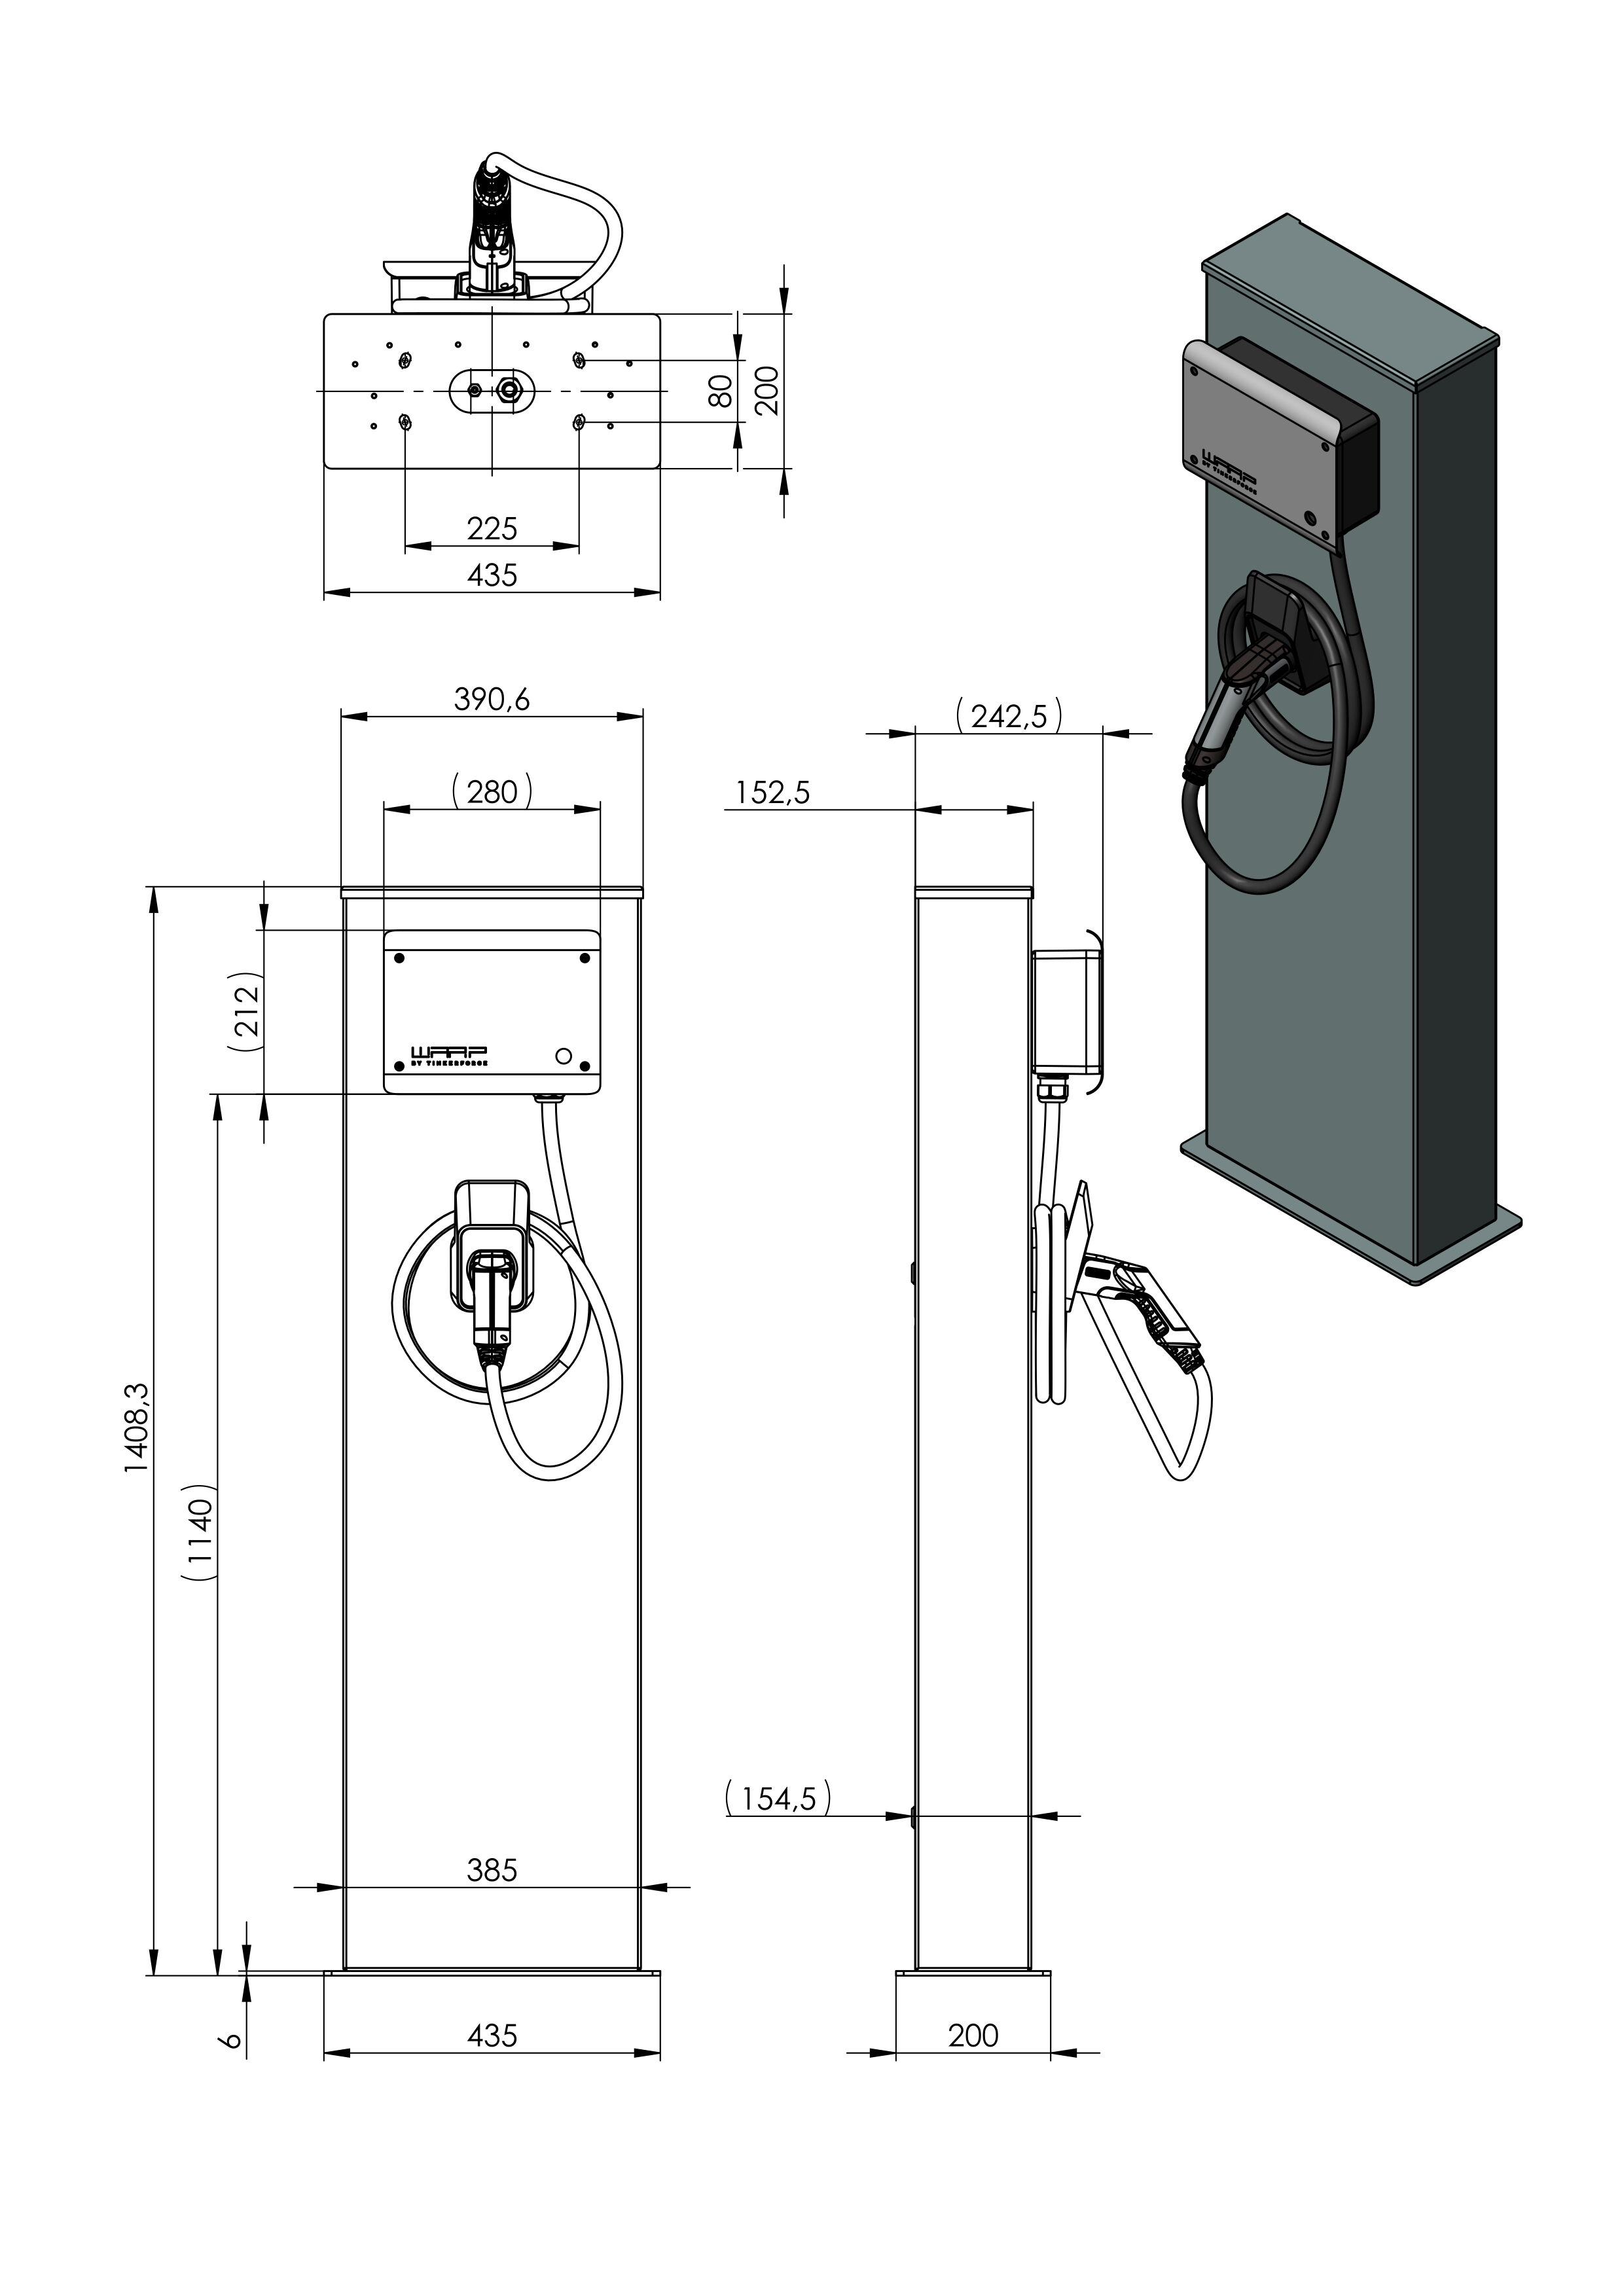
\includegraphics[width=0.9\linewidth]{./img4/stand.jpg}
	\end{center}


\end{document}
